\section{Theoretical Analysis}
\label{sec:analysis}

In this section we will analyse theoretical our bandpass filter using OP AMP. \\
To do so, and because there were several things to be analysed, we divided the theoretical analysis in the following subsections that explain the different sectors that our circuit has and also each one will be detailed separately.\\

\subsection{Transfer function computation}

In this section, a theoretical analysis of the circuit shown in section 1 was conducted. The OP Amp was considered ideal (internal impedance between v+ and v- is infinite, which means no current flows through it and vos=0 or in other words v+ = v-). So, in order to build a bass pand filter, a capacitor was connected in series (C1) with the input voltage which will function as a high pass filter (for low frequencies, the impedance goes to infinity and the capacitor is basically an open circuit)  and other capacitor (C2) was connected in parallel with the output voltage, functioning as a low pass filter (for high impedances, the impedance goes to 0 and the capacitor is basically a short circuit). To sum up, this circuit consists of a high pass filter, a signal amplifier and a low pass filter in series.

To compute the overall transfer function for this circuit we've computed the transfer function for these three stages and multiplied them all to obtain the overall transfer function.

\subsubsection{High pass filter stage}

\begin{figure}[H] 
\centering
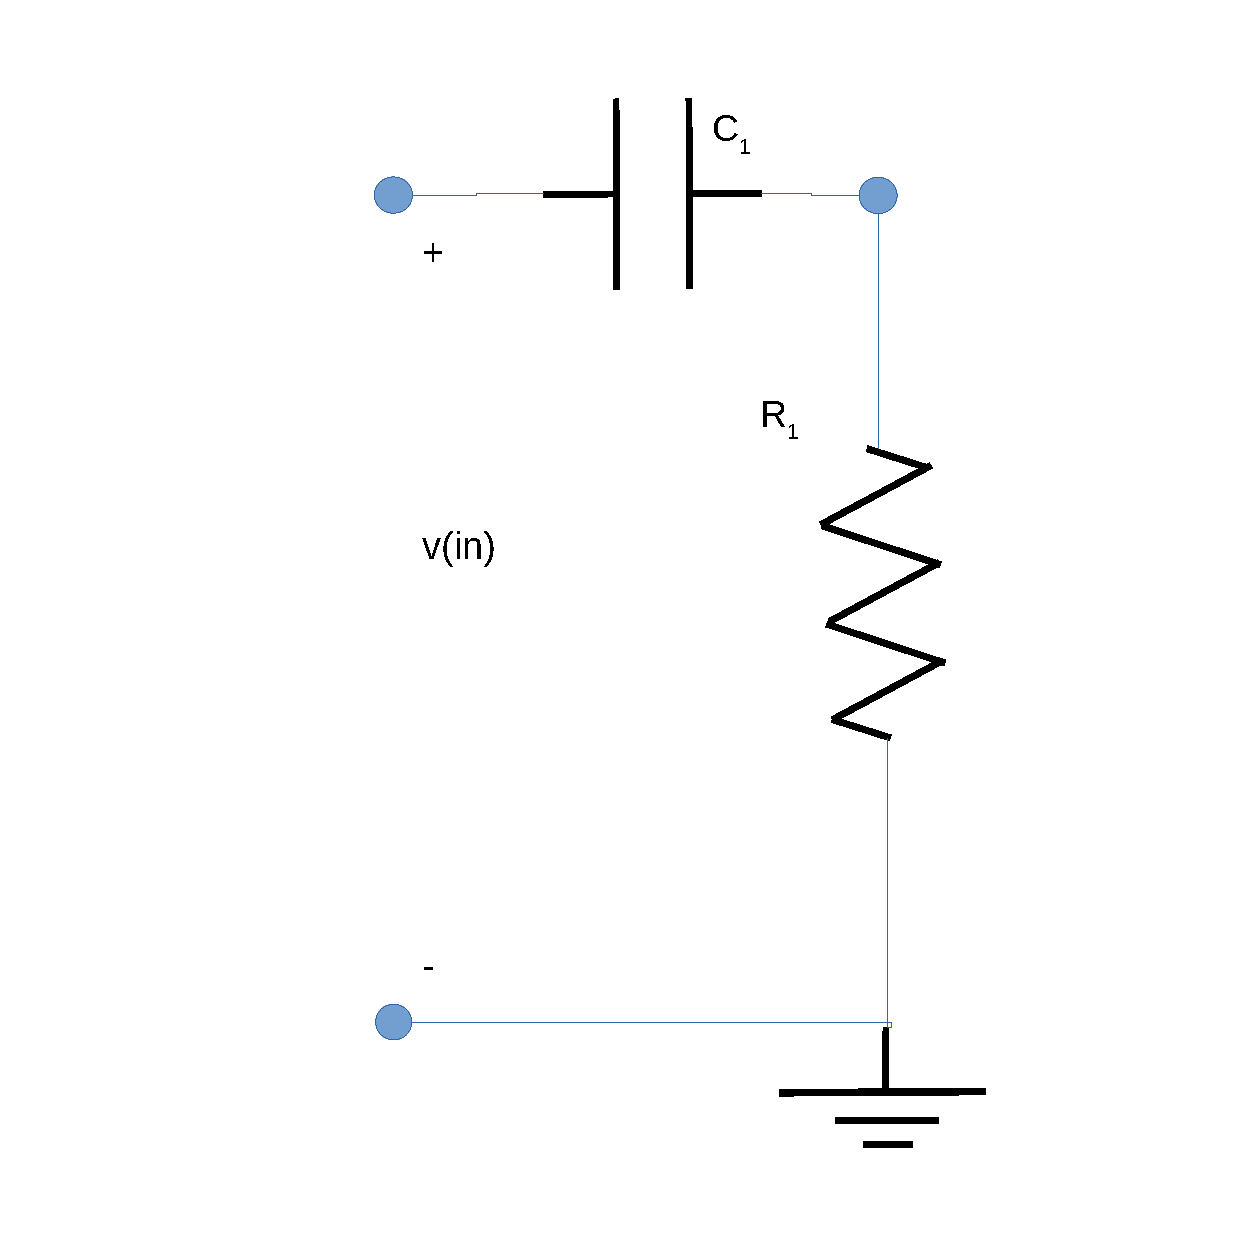
\includegraphics[width= 7cm]{high_pass_l5.pdf} 
\caption{High Pass Filter stage circuit}
\label{hf}
\end{figure}

Observing the image above and knowing that the input impedance at the op-amp is infinite, by just doing the voltage divider we've obtained the transfer function for this stage:

\begin{equation}
T_1(s) = \frac{R_1}{R_1 + \frac{1}{sC_1}} = \frac{R_1C_1s}{1+R_1C_1s}
\end{equation}   

\subsubsection{Gain stage}

\begin{figure}[H] 
\centering
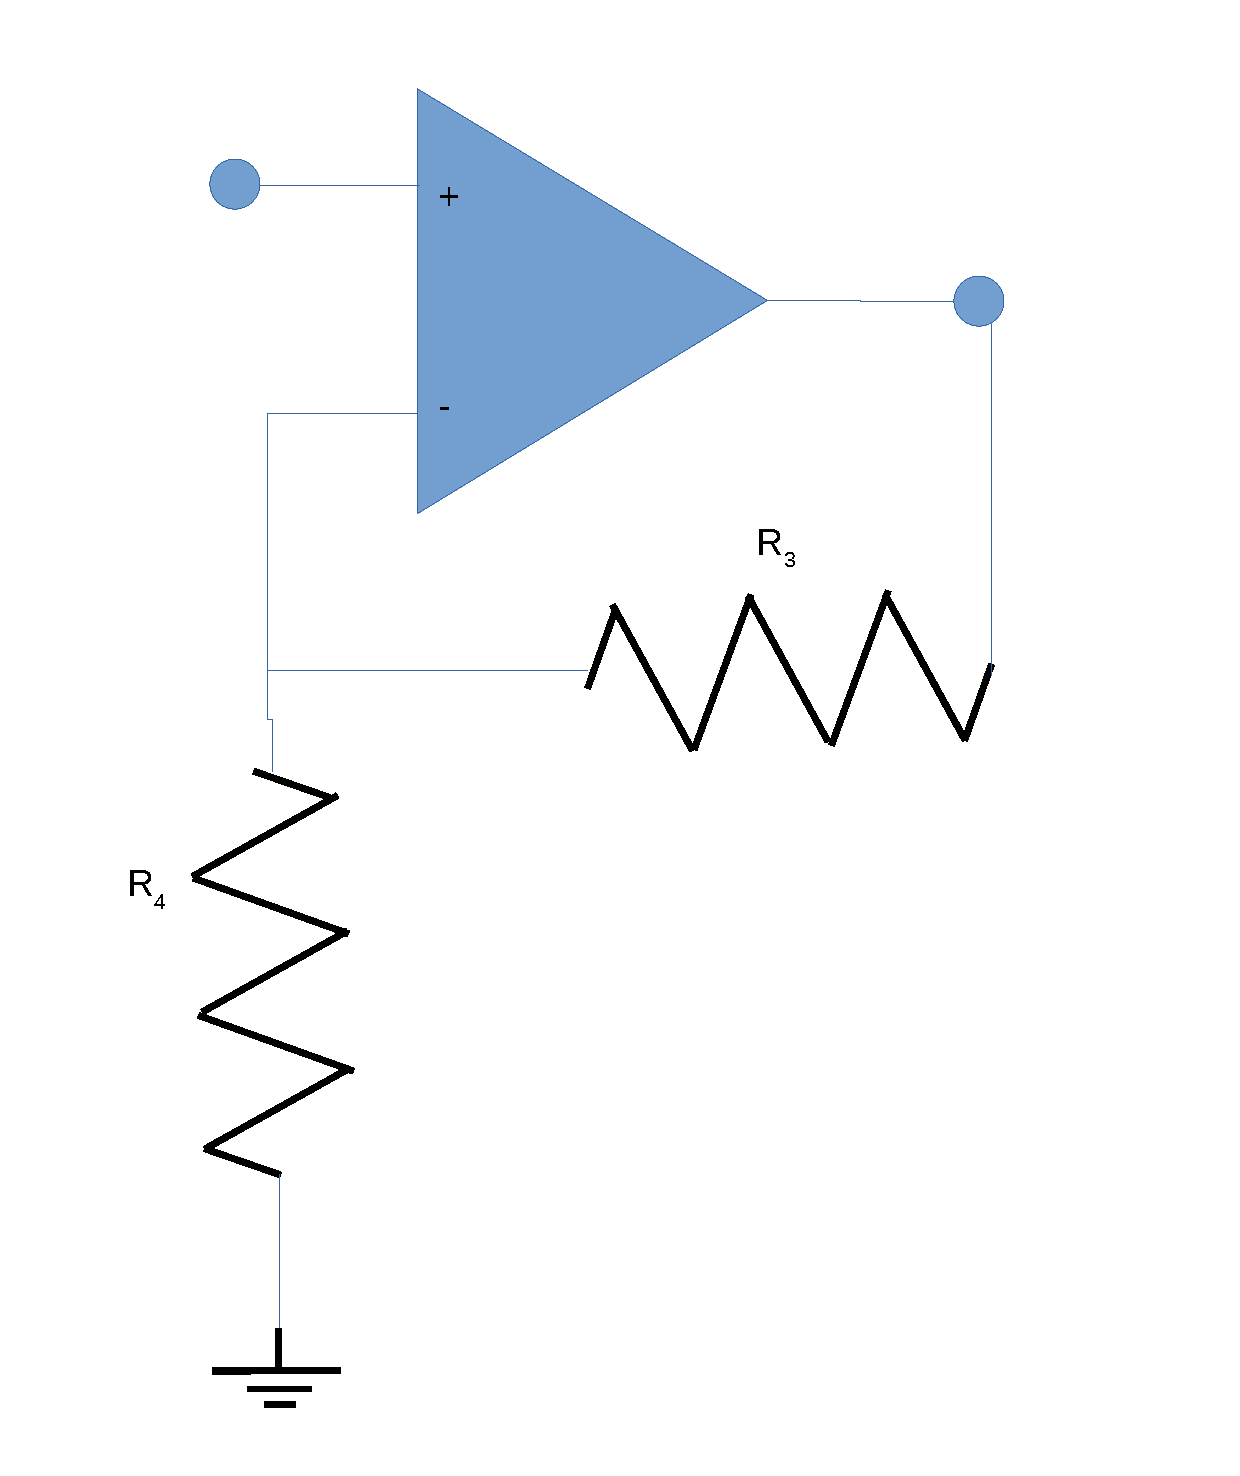
\includegraphics[width= 6cm]{amp_l5.pdf} 
\caption{Gain stage circuit}
\label{gainstage}
\end{figure}

To analyse these part of the circuit, first we need to specify some equations for the OP-Amp. 
Firstly the voltage in the two terminals is equal, which is, $v_3 = v_2$, and the other important thing to know is that the input impedance of this device is infinite. By knowing this, we can quickly determine the output voltage, as shown below.

\begin{equation}
v_o = v_4 = v_2 + v_{R_3} = v_3 + v_{R_3} = v_i + v_{R_3}
\end{equation} 

\begin{equation}
v_i = v_{R_4} = R_4i \iff i = \frac{v_i}{R_4}
\end{equation}

\begin{equation}
v_{R_3} = R_3i = \frac{R_3}{R_4}v_i
\end{equation}

So the transfer function for this stage is:

\begin{equation}
T_2(s) = \frac{v_o}{v_i} = \frac{v_i + v_{R_3}}{v_i} = \frac{(1+\frac{R_3}{R_4})v_i}{v_i} = 1 + \frac{R_3}{R_4}
\end{equation} 

\subsubsection{Low pass filter stage}

\begin{figure}[H] 
\centering
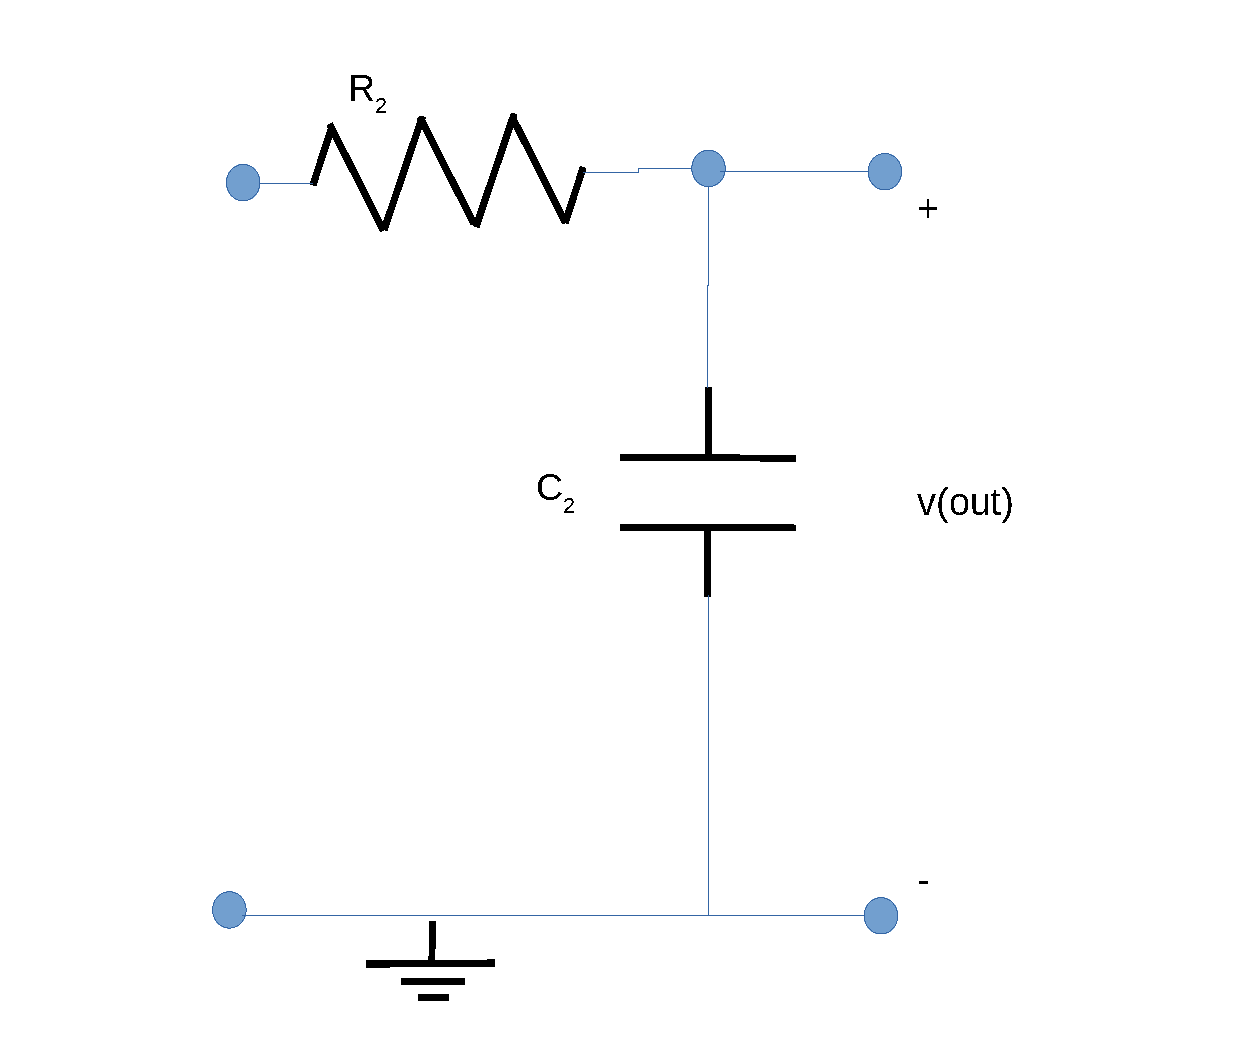
\includegraphics[width= 7cm]{low_pass_l5.pdf} 
\caption{Low pass filter stage circuit}
\label{lowpass}
\end{figure}

Once again, considering the figure above, by just making the voltage divider formulae we've obtained the transfer funcuntion for this stage.

\begin{equation}
T_3(s) = \frac{\frac{1}{sc_2}}{R_2 + \frac{1}{sc_2}} = \frac{1}{1+ C_2R_2s}
\end{equation} 

\subsubsection{Overall Transfer function}

The overall transfer function is given by:

\begin{equation}
T(s) = T_1(s)*T_2(s)*T_3(s) = \frac{R_1C_1s}{1+R_1C_1s}*(1 + \frac{R_3}{R_4})*\frac{1}{1+ C_2R_2s}
\end{equation} 

Using octave to plot this transfer function bode plots, we've obtain the following.

%FIGURE GAIN
\begin{figure}[H] 
\centering
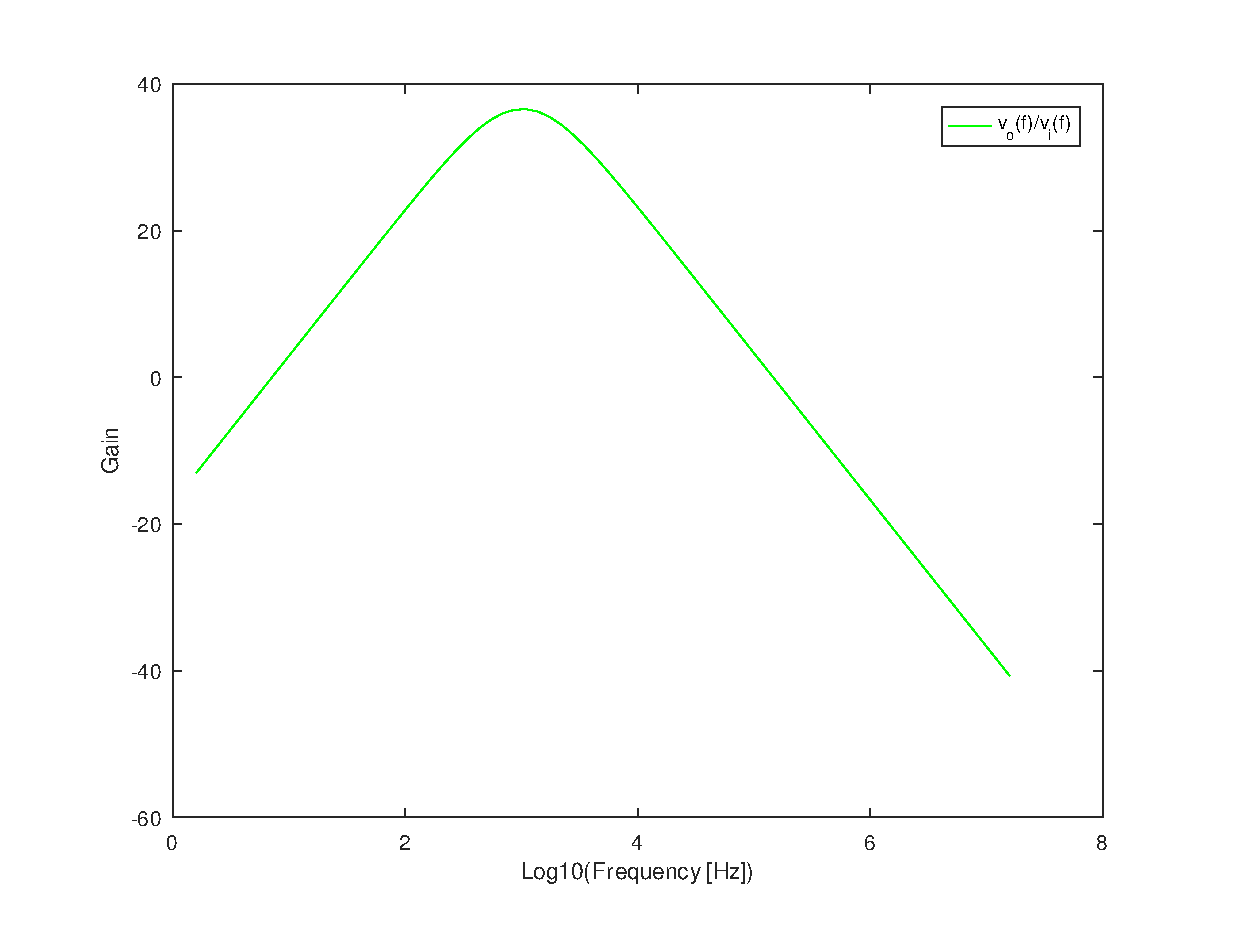
\includegraphics[width = 8cm]{gain.eps} 
\caption{Gain}
\label{gain}
\end{figure}

%FIGURE PHASE
\begin{figure}[H] 
\centering
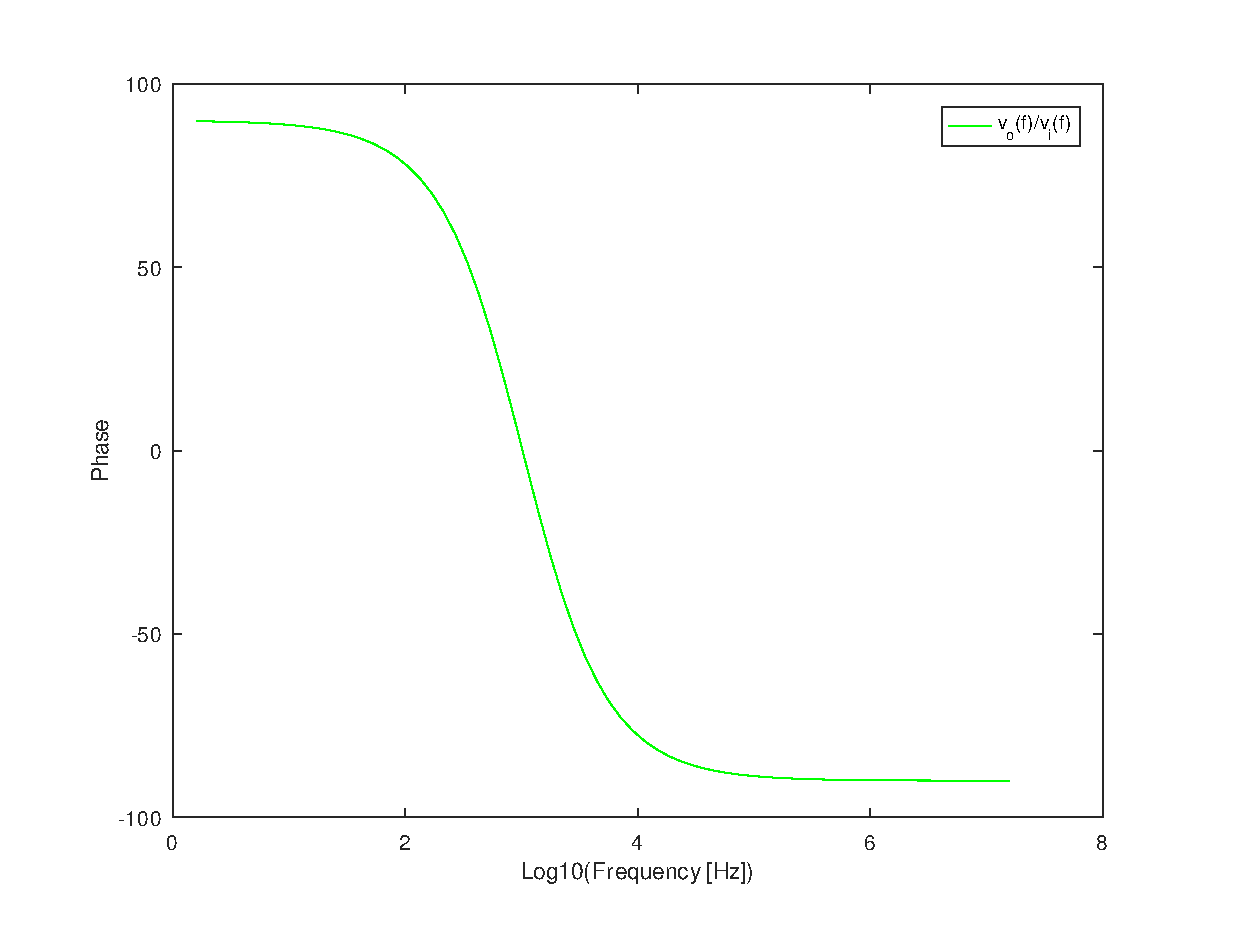
\includegraphics[width = 8cm]{phase.eps} 
\caption{Phase}
\label{phase}
\end{figure}

\subsection{Cutoff and Central Frequencies}

To obtain the cuttoff frequencies we just need to determine the poles of the transfer function. By looking at its formulae we obtain the following poles:

\begin{equation}
w_L = \frac{1}{R_1C_1}
\end{equation} 

\begin{equation}
w_H = \frac{1}{R_2C_2}
\end{equation} 

After obtaining these frequencies, in order to obtain the central frequency we just need to  obtain the frequency exatly in middle of these two cutoff frequencies in the gain plot in dB. This means that the central frequency is given by the following formulae:

\begin{equation}
w_0 = \sqrt{w_Lw_H}
\end{equation} 

Using octave we've reached the following values for these 3 frequencies.

%BANDPASS FREQUENCY
\begin{table}[H] \centering
\begin{tabular}{|
>{\columncolor[HTML]{FFCC67}}l |c|}
\hline
\multicolumn{2}{|l|}{\cellcolor[HTML]{EABD8B}Name - Value} \\ \hline
LowFreq BandPass & 4.545455e+03 \\ \hline
HighFreq BandPass & 9.090909e+03 \\ \hline
Central Freq & 6.428243e+03 \\ \hline

\end{tabular}
\caption{Band Pass Frequency}
\end{table}

With respect to the central frequency we've also obtained its value in Hz and its gain in dB 

%WO FREQUENCY GAIN
\begin{table}[H] \centering
\begin{tabular}{|
>{\columncolor[HTML]{FFCC67}}l |c|}
\hline
\multicolumn{2}{|l|}{\cellcolor[HTML]{EABD8B}Name - Value} \\ \hline
Central Freq (Hz) & 1.023087e+03 \\ \hline
Gain Central Freq (dB) & 3.656460e+01 \\ \hline

\end{tabular}
\caption{WO Frequency Gain}
\end{table}


\subsection{Input and Output Impedances}

In order to compute the input impedance we take the circuit and turn off all independent sources. After these we connect an independent voltage source in the input of the circuit and determine the current in these source. Observing the circuit in the introduction and knowing that the input impedance of the OP-Amp is infinite, we get that the input impedance is just the resistor $R_1$ and the capacitor $C_1$ in series, so the input impedance for the central frequency is:

\begin{equation}
Z_{in} = R_1 + \frac{1}{jw_0C_1}
\end{equation} 

To compute the output stage, we start in the same way as the input impedance, by turning off all the independent sources. After these, instead of connecting a independent voltage source at the input of the circuit, we connect it to the output, and determine the current at these source in the same way as before. Because the output impedance of the OP-Amp is 0, the output impedance of the circuit is just the resistor $R_2$ and the capacitor $C_2$ in parallel. So the output uimpedance for the central frequency is given by:

\begin{equation}
Z_{out} = \frac{R_2}{1 + jR_2C_2w_0}
\end{equation} 

Using octave, we've obtain the following values for the impedances:

%IMPEDANCES
\begin{table}[H] \centering
\begin{tabular}{|
>{\columncolor[HTML]{FFCC67}}l |c|}
\hline
\multicolumn{2}{|l|}{\cellcolor[HTML]{EABD8B}Name - Value} \\ \hline
Z in & 1.000000e+03 + -7.071068e+02j \\ \hline
Z out & 6.666667e+02 + -4.714045e+02j\\ \hline

\end{tabular}
\caption{Impedances}
\end{table}


